\chapter{HASIL DAN PEMBAHASAN}

\vspace{1cm}
\section{Area Studi}
\hspace{1,2cm}
Terdapat dua area studi yang dilakukan pada penelitian ini, yaitu Kebun Pendidikan dan Penelitian Kelapa Sawit milik Institut Pertanian Bogor-Cargil yang berlokasi di Jonggol, Jawa Barat dan Universitas Gunadarma di Penajam Paser Utara, Kalimantan Timur yang memiliki lahan yang ditanami pohon kelapa sawit.

Area studi ini secara umum mencakup untuk pengambilan data citra pohon kelapa sawit sebagai dataset primer. Tabel \ref{tbl:Data-Lokasi-dan-Luasan-Area-Studi} menampilkan lokasi koordinat dan luasan lahan yang diambil sebagai citra pohon kelapa sawit.

%%%%%%%%%%%%%%%%%%%%%%%TABEL SEDERHANA%%%%%%%%%%%%%%%%%%%%%%%%%
\begin{singlespace}
	\begin{table}[H]
		\centering
		\caption{Data Lokasi dan Luasan Area Studi}
		\label{tbl:Data-Lokasi-dan-Luasan-Area-Studi}
		\begin{tabular}{|p{4cm}|p{4cm}|p{4cm}|}
			\hline
			\rowcolor[HTML]{D9D9D9}
			Area Studi                                                                         & Lokasi Koordinat (Latitude, Longitude) & Luasan Lahan (ha) \\ \hline

			Kebun Pendidikan dan Penelitian Kelapa Sawit milik Institut Pertanian Bogor-Cargil & -6.4277942, 106.8418378                                                          & 63,48                                                          \\ \hline
			
			Universitas Gunadarma di Penajam Paser Utara, Kalimantan Timur                     & -1.318495, 116.6678405                                                           & $\approx$ 18                                                           \\ \hline
			\end{tabular}
	\end{table}
\end{singlespace}
%%%%%%%%%%%%%%%%%%%%%%%TABEL SEDERHANA%%%%%%%%%%%%%%%%%%%%%%%%%

Pengambilan citra pada area studi diambil dengan menggunakan DJI Mavic 2 Pro dari ketinggian 100 m di atas permukaan tanah dengan pakar atau pilot drone yang sudah tersertifikasi. Pada tahap pengujian pada sistem untuk mendeteksi dan menghitung, serta titik koordinat latitude-longitude dari setiap pohon kelapa sawit menggunakan area Kebun Pendidikan dan Penelitian Kelapa Sawit milik Institut Pertanian Bogor-Cargil Blok 1, 2, 3, dan 4. Pada proses pengambilan citra untuk dataset primer pada area studi lahan pada Kebun Pendidikan dan Penelitian Kelapa Sawit milik Institut Pertanian Bogor-Cargil berhasil ditangkap area blok 3 dan 4 dari total 4 blok. Peta sebaran area inisialisasi lahan pada kebun ini seperti pada Gambar \ref{img:Peta-Sebaran-Area-Inisialisasi-Lahan-Kebun} yang memiliki 5670 pohon tanam kelapa sawit berdasarkan hasil wawancara di lapangan pada area studi Kebun Pendidikan dan Penelitian Kelapa Sawit milik Institut Pertanian Bogor-Cargil.

%%%%%%%%%%%%%%%%%%%%%%%%%% GAMBAR %%%%%%%%%%%%%%%%%%%%%%%%%%%%%%
\begin{figure}[H]
	\vspace{-0.1cm}
	%\rule{\columnwidth}{0.1pt}
	\begin{center}
		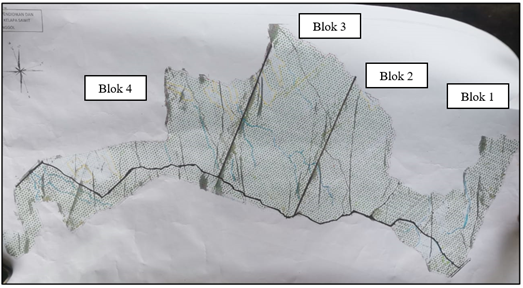
\includegraphics[width=1\columnwidth]{bab4/Gambar/Picture1.png}
	\end{center}
	\vspace{-0.2cm}
	%\rule{\columnwidth}{0.1pt}
	\captionsetup{justification=centering}
	\caption{Peta Sebaran Area Inisialisasi Lahan Kebun Pendidikan dan Penelitian Kelapa Sawit milik Institut Pertanian Bogor-Cargil}\label{img:Peta-Sebaran-Area-Inisialisasi-Lahan-Kebun}
\end{figure}
%%%%%%%%%%%%%%%%%%%%%%%%%% GAMBAR %%%%%%%%%%%%%%%%%%%%%%%%%%%%%%

Area lahan yang berhasil ditangkap pada kebun ini berada pada area studi blok 3 dan blok 4. Area studi yang digunakan untuk dataset primer yang digunakan blok 3 pada Gambar 3.6 dan blok 4 pada Gambar 3.7. dengan total luas sebesar 37,51 hektar, dan pengujian digunakan blok 1 (Gambar 4.2), 2 (Gambar 4.3), 3, dan 4 seperti pada Tabel \ref{tbl:Area-Studi-Yang-Berhasil-Ditangkap-Menjadi-CItra-Area-Pohon-Kelapa-Sawit-Dengan-Drone} dengan total luas area 63,48 hektar pada Kebun Pendidikan dan Penelitian Kelapa Sawit Institut Pertanian Bogor-Cargil dengan perhitungan luas area menggunakan bantuan layanan DroneDeploy.

%%%%%%%%%%%%%%%%%%%%%%%TABEL SEDERHANA%%%%%%%%%%%%%%%%%%%%%%%%%
\begin{singlespace}
	\begin{table}[H]
		\centering
		\caption{Area Studi yang Berhasil Ditangkap menjadi Citra Area Pohon Kelapa Sawit dengan Drone}
		\label{tbl:Area-Studi-Yang-Berhasil-Ditangkap-Menjadi-CItra-Area-Pohon-Kelapa-Sawit-Dengan-Drone}
		\begin{tabular}{|ll|l|}
			\hline
			\rowcolor[HTML]{D9D9D9} 
			\multicolumn{1}{|l|}{\cellcolor[HTML]{D9D9D9}No.} & Area   & Luas Area (ha) \\ \hline
			\multicolumn{1}{|l|}{1}                           & Blok 1 & 14,66          \\ \hline
			\multicolumn{1}{|l|}{2}                           & Blok 2 & 11,31          \\ \hline
			\multicolumn{1}{|l|}{3}                           & Blok 3 & 18,20          \\ \hline
			\multicolumn{1}{|l|}{4}                           & Blok 4 & 19,31          \\ \hline
			\multicolumn{2}{|l|}{Total}                                & 63,48          \\ \hline
		\end{tabular}
	\end{table}
\end{singlespace}
%%%%%%%%%%%%%%%%%%%%%%%TABEL SEDERHANA%%%%%%%%%%%%%%%%%%%%%%%%%

%%%%%%%%%%%%%%%%%%%%%%%%%% GAMBAR %%%%%%%%%%%%%%%%%%%%%%%%%%%%%%
\begin{figure}[H]
	\vspace{-0.1cm}
	%\rule{\columnwidth}{0.1pt}
	\begin{center}
		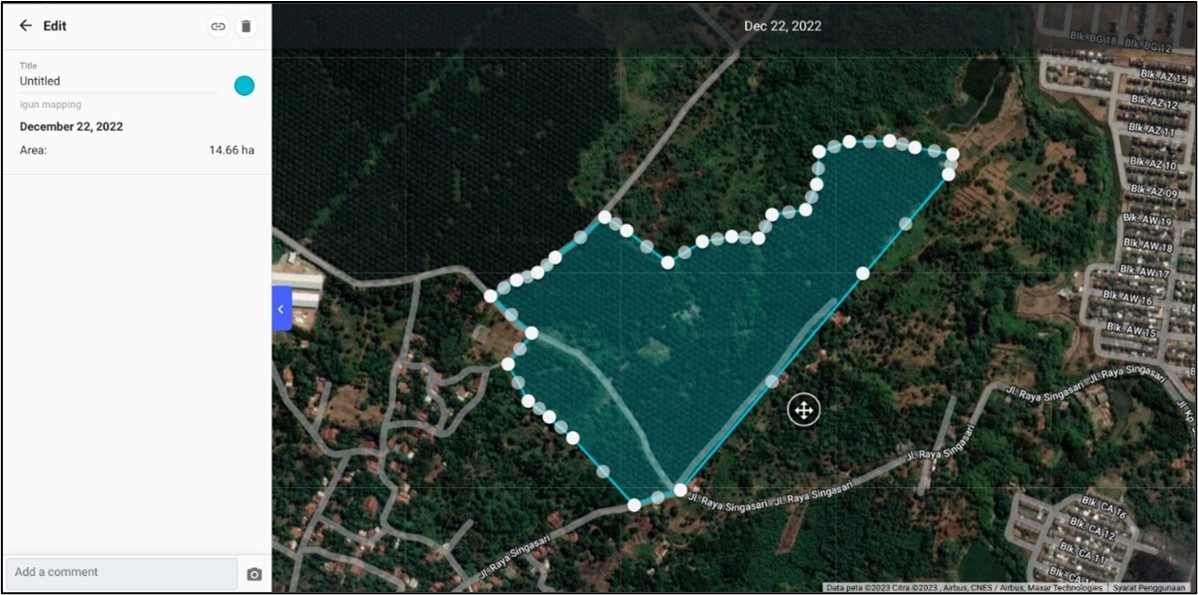
\includegraphics[width=0.7\columnwidth]{bab4/Gambar/Picture2.jpg}
	\end{center}
	\vspace{-0.2cm}
	%\rule{\columnwidth}{0.1pt}
	\captionsetup{justification=centering}
	\caption{Luas Area Blok 1 Kebun Pendidikan dan Penelitian Kelapa Sawit Institut Pertanian Bogor-Cargil}\label{img:Luas-Area-Blok-1-Kebun-Pendidikan}
\end{figure}
%%%%%%%%%%%%%%%%%%%%%%%%%% GAMBAR %%%%%%%%%%%%%%%%%%%%%%%%%%%%%%

%%%%%%%%%%%%%%%%%%%%%%%%%% GAMBAR %%%%%%%%%%%%%%%%%%%%%%%%%%%%%%
\begin{figure}[H]
	\vspace{-0.1cm}
	%\rule{\columnwidth}{0.1pt}
	\begin{center}
		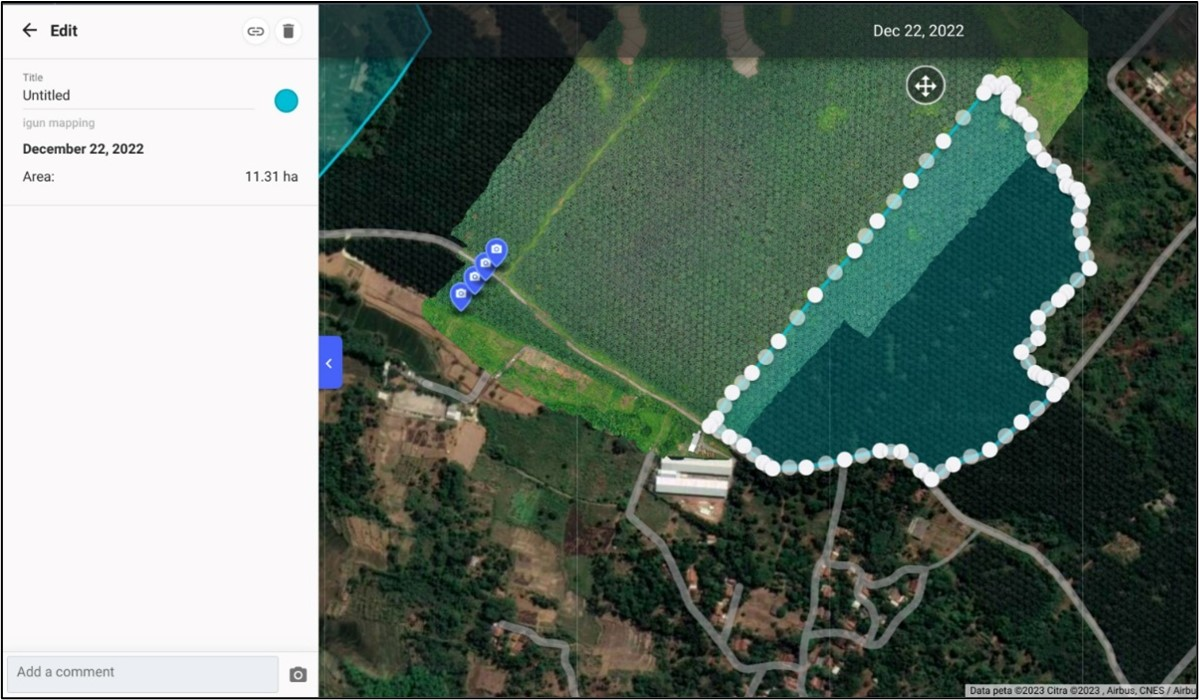
\includegraphics[width=0.7\columnwidth]{bab4/Gambar/Picture3.jpg}
	\end{center}
	\vspace{-0.2cm}
	%\rule{\columnwidth}{0.1pt}
	\captionsetup{justification=centering}
	\caption{Luas Area Blok 2 Kebun Pendidikan dan Penelitian Kelapa Sawit Institut Pertanian Bogor-Cargil}\label{img:Luas-Area-Blok-2-Kebun-Pendidikan}
\end{figure}
%%%%%%%%%%%%%%%%%%%%%%%%%% GAMBAR %%%%%%%%%%%%%%%%%%%%%%%%%%%%%%

\section{Persiapan Data}
\hspace{1,2cm}
Persiapan data, yang dikenal dengan \textit{data preprocessing} adalah tahap yang penting untuk menyiapkan data untuk dapat digunakan dalam modeling dengan \textit{deep learning}. Persiapan data meliputi persiapan dataset primer dan sekunder untuk dapat digunakan.

\subsection{Deskripsi Dataset dan Pemilihan}
\hspace{1,2cm}
Akuisisi citra area pohon kelapa sawit menjadi penting karena berhubungan hasil memindai, menangkap (\textit{capture}), atau menjadi suatu foto citra yang dapat digunakan untuk dataset. Citra area pohon kelapa sawit pada penelitian ini dibagi menjadi dua, yaitu citra untuk dataset primer dan sekunder.

\subsubsection{Dataset Primer}
\hspace{1,2cm}
Dataset primer digunakan untuk membangun atau memberikan anotasi atau label oil palm pada citra gambar. Hasil gambar citra pohon kelapa sawit dari dua area studi memiliki format citra yang sama, yaitu *.jpg. Data citra dari Kebun Pendidikan dan Penelitian Kelapa Sawit milik Institut Pertanian Bogor-Cargil yang diambil dari blok 3 dan 4 terdiri dari 69 citra atau gambar, sedangkan jumlah citra yang dihasilkan dari area kelapa sawit berjumlah 205 citra dengan dimensi ukuran citra sebesar 5472 x 3078 px, seperti pada Tabel \ref{tbl:Jumlah-Citra-Dari-Dua-Area-Studi}

Total citra dataset primer dari dua area studi seperti pada Tabel \ref{tbl:Jumlah-Citra-Dari-Dua-Area-Studi} berikut.

%%%%%%%%%%%%%%%%%%%%%%%TABEL SEDERHANA%%%%%%%%%%%%%%%%%%%%%%%%%
\begin{singlespace}
	\begin{table}[H]
		\centering
		\caption{Jumlah Citra dari Dua Area Studi}
		\label{tbl:Jumlah-Citra-Dari-Dua-Area-Studi}
		\begin{tabular}{|p{4cm}|p{4cm}|p{4cm}|}
			\hline
			\rowcolor[HTML]{D9D9D9} 
			Area Studi                                                                         & Jumlah Citra & Luas Area (ha) \\ \hline
			Kebun Pendidikan dan Penelitian Kelapa Sawit milik Institut Pertanian Bogor-Cargil & 69           & 14,66          \\ \hline
			Universitas Gunadarma di Penajam Paser Utara, Kalimantan Timur                     & 205          & 11,31          \\ \hline
		\end{tabular}
	\end{table}
\end{singlespace}
%%%%%%%%%%%%%%%%%%%%%%%TABEL SEDERHANA%%%%%%%%%%%%%%%%%%%%%%%%%

Hasil citra dari area studi Universitas Gunadarma dengan jumlah 205 citra atau gambar ini digunakan untuk dataset primer dengan memberikan anotasi atau pemberian label secara otomatis yang dilakukan dalam penelitian ini.  Adapun citra sampel area studi dari Universitas Gunadarma tampak pada Gambar \ref{img:Hasil-Citra-Sampel-Universitas-Gunadarma-1} dan citra sampel Kebun Pendidikan dan Penelitian Kelapa Sawit milik Institut Pertanian Bogor-Cargil tampak pada Gambar \ref{img:Hasil-Citra-Sampel-Universitas-Gunadarma-2}

%%%%%%%%%%%%%%%%%%%%%%%%%% GAMBAR %%%%%%%%%%%%%%%%%%%%%%%%%%%%%%
\begin{figure}[H]
	\vspace{-0.1cm}
	%\rule{\columnwidth}{0.1pt}
	\begin{center}
		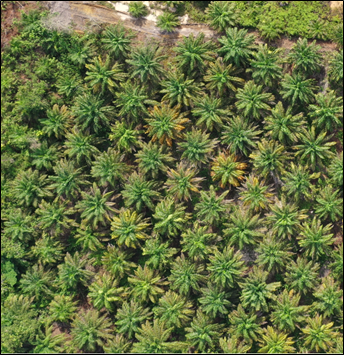
\includegraphics[width=0.6\columnwidth]{bab4/Gambar/Picture4.1.png}
		\hspace{1cm}
		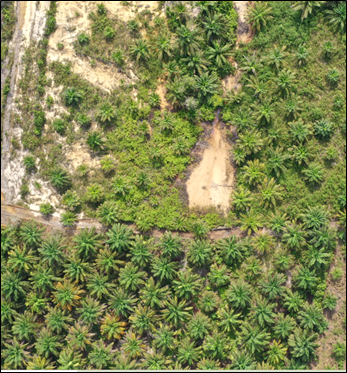
\includegraphics[width=0.6\columnwidth]{bab4/Gambar/Picture4.2.png}
	\end{center}
	\vspace{-0.2cm}
	%\rule{\columnwidth}{0.1pt}
	\captionsetup{justification=centering}
	\caption{Hasil Citra Sampel Universitas Gunadarma di Penajam Paser Utara, Kalimantan Timur}\label{img:Hasil-Citra-Sampel-Universitas-Gunadarma-1}
\end{figure}
%%%%%%%%%%%%%%%%%%%%%%%%%% GAMBAR %%%%%%%%%%%%%%%%%%%%%%%%%%%%%%

%%%%%%%%%%%%%%%%%%%%%%%%%% GAMBAR %%%%%%%%%%%%%%%%%%%%%%%%%%%%%%
\begin{figure}[H]
	\vspace{-0.1cm}
	%\rule{\columnwidth}{0.1pt}
	\begin{center}
		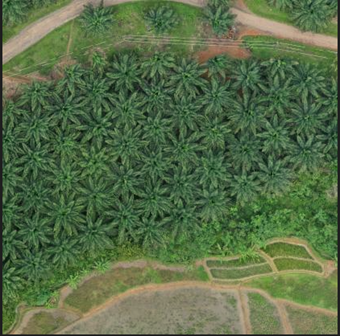
\includegraphics[width=0.6\columnwidth]{bab4/Gambar/Picture5.1.png}
		\hspace{1cm}
		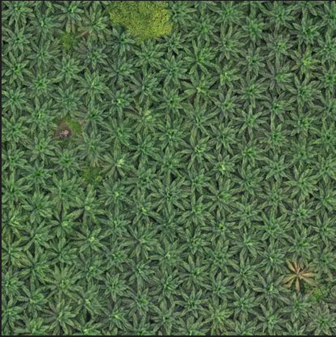
\includegraphics[width=0.6\columnwidth]{bab4/Gambar/Picture5.2.png}
	\end{center}
	\vspace{-0.2cm}
	%\rule{\columnwidth}{0.1pt}
	\captionsetup{justification=centering}
	\caption{Hasil Citra Sampel Universitas Gunadarma di Penajam Paser Utara, Kalimantan Timur}\label{img:Hasil-Citra-Sampel-Universitas-Gunadarma-2}
\end{figure}
%%%%%%%%%%%%%%%%%%%%%%%%%% GAMBAR %%%%%%%%%%%%%%%%%%%%%%%%%%%%%%

\subsubsection{Dataset Sekunder}
\hspace{1,2cm}
Data sekunder yang digunakan sudah memiliki label atau anotasi sebagai pohon kelapa sawit "oil palm". Data berjumlah 1795 citra yang sudah memiliki kotak batas atau \textit{bounding box} dengan kelas \textit{oil palm}. Data sekunder digunakan untuk menambah data pada sata proses pelatihan, validasi dan pengujian. Data tersebut semakin bervariasi, maka keterwakilan data pada citra yang berupa objek pohon kelapa sawit semakin baik. Dataset sekunder dapat diakses secara daring dan dapat digunakan secara \textit{free} atau \textit{open source} melalui sistem berbasis web bernama roboflow.

GAMBAR

Data sample pada dataset sekunder yang sudah memiliki \textit{bounding box} yang diberi label oil palm, seperti pada Gambar 4.6.

Dataset sekunder ini dilakukan proses augmentasi dengan menggunakan bantuan layanan roboflow. Proses augmentasi ini dilakukan untuk menambah banyaknya data citra, serta bertujuan agar mesin dapat belajar dan mengenali dari berbagai citra yang berbeda-beda. Penggunaan augmentasi ini diharapkan dapat meningkatkan performa dari model, karena mesin yang digunakan dalam penelitian ini agar dapat berhasil mengenali lebih banyak objek dari bentuk dan pola yang beragam jenis data citra. 

Data sekunder ini berada pada layanan roboflow dan memiliki fasilitas layanan untuk augmentasi. Proses augmentasi dilakukan dengan menambahkan data citra dari data sekunder, seperti pada Gambar 4.7.

%%%%%%%%%%%%%%%%%%%%%%%%%% GAMBAR %%%%%%%%%%%%%%%%%%%%%%%%%%%%%%
\begin{figure}[H]
	\vspace{-0.1cm}
	%\rule{\columnwidth}{0.1pt}
	\begin{center}
		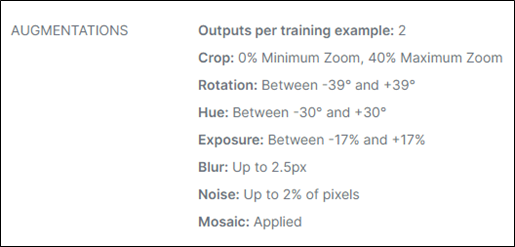
\includegraphics[width=1\columnwidth]{bab4/Gambar/Picture7.png}
	\end{center}
	\vspace{-0.2cm}
	%\rule{\columnwidth}{0.1pt}
	\captionsetup{justification=centering}
	\caption{Proses Augmentasi Data Sekunder }\label{img:Proses-Augmentasi-Data-Sekunder}
\end{figure}
%%%%%%%%%%%%%%%%%%%%%%%%%% GAMBAR %%%%%%%%%%%%%%%%%%%%%%%%%%%%%%

Fitur layanan augmentasi yang digunakan antara lain \textit{crop, rotation, hue, exposure, blur, noise, dan mosaic}. Fitur layanan ini memiliki kegunaan yang mewakili kondisi seperti data studi atau lapangan. Kegunaan fitur layanan yang digunakan seperti pada Tabel \ref{tbl:Kegunaan-Layanan-Augmentasi-Dataset-Sekunder}.
	
%%%%%%%%%%%%%%%%%%%%%%%TABEL SEDERHANA%%%%%%%%%%%%%%%%%%%%%%%%%
\begin{singlespace}
	\begin{table}[H]
		\centering
		\caption{Kegunaan Layanan Augmentasi Dataset Sekunder}
		\label{tbl:Kegunaan-Layanan-Augmentasi-Dataset-Sekunder}
		\begin{tabular}{|p{3cm}|p{8cm}|}
			\hline
			\rowcolor[HTML]{D9D9D9} 
			Augmentasi & Kegunaan                                                                                                                                             \\ \hline
			Crop       & Menambahkan variabilitas pada pemosisian dan ukuran untuk membantu model lebih mengenali terhadap translasi subjek dan posisi kamera.                \\ \hline
			Rotation   & Menambahkan variabilitas pada rotasi untuk membantu model agar dapat mendeteksi objek, bahkan saat kamera atau subjek tidak sejajar secara sempurna. \\ \hline
			Hue        & Mengubah warna secara acak untuk membuat model tidak terlalu sensitif.                                                                       \\ \hline
			Exposure & Menambahkan variabilitas pada kecerahan gambar untuk membantu model lebih dapat mengenali terhadap perubahan pencahayaan dan pengaturan kamera. \\ \hline
			Blur & Menambahkan keburaman Gaussian secara acak untuk membantu model lebih mengenali terhadap fokus kamera, jika data citra berada pada area hutan, kebun, dan alam liar, mungkin tidak berada dalam keadaan focus tangkapan citra tersebut. \\ \hline
			Noise & Menambahkan noise untuk membantu model lebih mengenali terhadap noise yang dapat membantu mempertahankan nilai dan menghindari overfitting dari hasil pengujian. \\ \hline
			Mosaic & Menambahkan mosaik untuk membantu model tampil lebih baik pada objek kecil, mosaik menggabungkan beberapa foto dari rangkaian pelatihan data. \\ \hline
		\end{tabular}
	\end{table}
\end{singlespace}
%%%%%%%%%%%%%%%%%%%%%%%TABEL SEDERHANA%%%%%%%%%%%%%%%%%%%%%%%%%

Tabel 4.5 . menampilkan hasil data citra untuk dataset yang telah dilakukan proses augmentasi sesuai dengan Tabel 4.4. dan tampalian data citra yang berbeda dengan data citra dataset sekunder asli seperti pada Gambar \ref{img:Data-Citra-Asli-Data-Sekunder}.

%%%%%%%%%%%%%%%%%%%%%%%%%% GAMBAR %%%%%%%%%%%%%%%%%%%%%%%%%%%%%%
\begin{figure}[H]
	\vspace{-0.1cm}
	%\rule{\columnwidth}{0.1pt}
	%\begin{center}
	%	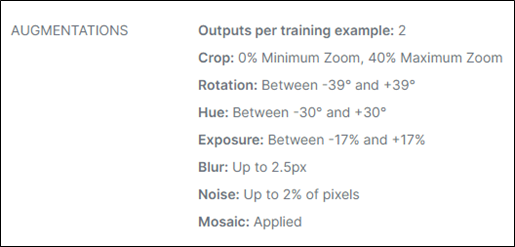
\includegraphics[width=1\columnwidth]{bab4/Gambar/Picture7.png}
	%\end{center}
	\centering
	\subfloat{{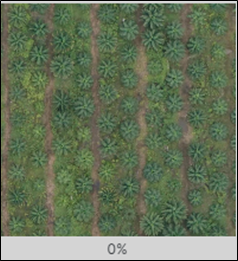
\includegraphics[width=6cm]{bab4/Gambar/Picture8.1.png} }}%
	\qquad
	\subfloat{{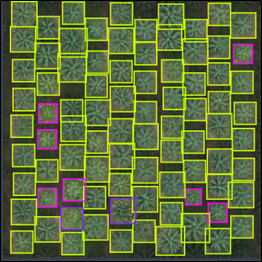
\includegraphics[width=6cm]{bab4/Gambar/Picture8.2.png} }}%
	\vspace{-0.2cm}
	%\rule{\columnwidth}{0.1pt}
	\captionsetup{justification=centering}
	\caption{Data Citra Asli Data Sekunder (kiri: original; kanan: tampak dengan \textit{bounding box}) }\label{img:Data-Citra-Asli-Data-Sekunder}
\end{figure}
%%%%%%%%%%%%%%%%%%%%%%%%%% GAMBAR %%%%%%%%%%%%%%%%%%%%%%%%%%%%%%

%%%%%%%%%%%%%%%%%%%%%%%TABEL SEDERHANA%%%%%%%%%%%%%%%%%%%%%%%%%
\begin{singlespace}
	\begin{table}[H]
		\centering
		\caption{Hasil Proses Augmentasi Citra Dataset Sekunder}
		\label{tbl:Hasil-Proses-Augmentasi-Citra-Dataset-Sekunder}
		\begin{tabular}{|m{3cm}|m{3cm}|m{6cm}|}
			\hline
			\rowcolor[HTML]{D9D9D9} 
			Augmentasi & Deskripsi                                                                & Citra Hasil Augmentasi \\ \hline
			
			
			Crop & 0\% Minimum Zoom,\newline 40\% Maximum Zoom & 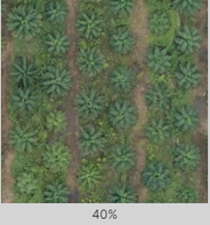
\includegraphics[width=0.4\columnwidth]{bab4/Gambar/tbl-5-pic1.png}\\ \hline
			
			Rotation & Between -39$^{\circ}$ and +39$^{\circ}$ & 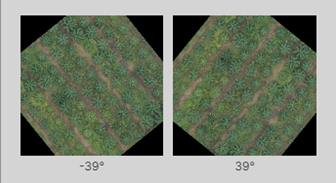
\includegraphics[width=0.4\columnwidth]{bab4/Gambar/tbl-5-pic2.png}\\ \hline
		\end{tabular}
	\end{table}
\end{singlespace}
%%%%%%%%%%%%%%%%%%%%%%%TABEL SEDERHANA%%%%%%%%%%%%%%%%%%%%%%%%%

%%%%%%%%%%%%%%%%%%%%%%%TABEL SEDERHANA%%%%%%%%%%%%%%%%%%%%%%%%%
\begin{singlespace}
	\begin{table}[H]
		\centering
		%\caption{Hasil Proses Augmentasi Citra Dataset Sekunder}
		%\label{tbl:Hasil-Proses-Augmentasi-Citra-Dataset-Sekunder}
		\begin{tabular}{|m{3cm}|m{3cm}|m{6cm}|}
			\hline
			\rowcolor[HTML]{D9D9D9} 
			Augmentasi & Deskripsi                                                                & Citra Hasil Augmentasi \\ \hline
			
			
			Hue & 0\% Between -30$^{\circ}$ and +30$^{\circ}$ & 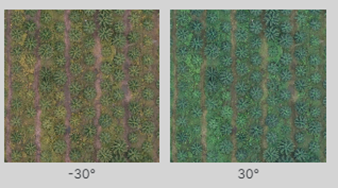
\includegraphics[width=0.4\columnwidth]{bab4/Gambar/tbl-5-pic3.png}\\ \hline
			
			Exposure & Between -17$^{\circ}$ and +17$^{\circ}$ & 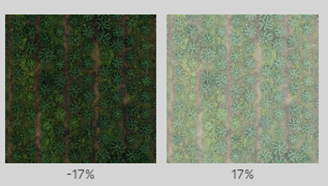
\includegraphics[width=0.4\columnwidth]{bab4/Gambar/tbl-5-pic4.png}\\ \hline
			
			Blur & Up to 2.5px & 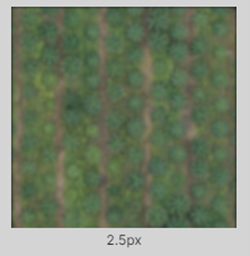
\includegraphics[width=0.4\columnwidth]{bab4/Gambar/tbl-5-pic5.png}\\ \hline
			
			Noise & Up to 2\% of pixels & 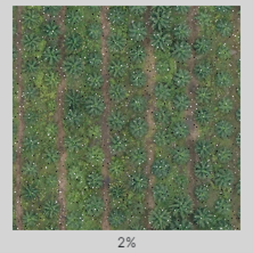
\includegraphics[width=0.4\columnwidth]{bab4/Gambar/tbl-5-pic6.png}\\ \hline
		\end{tabular}
	\end{table}
\end{singlespace}
%%%%%%%%%%%%%%%%%%%%%%%TABEL SEDERHANA%%%%%%%%%%%%%%%%%%%%%%%%%

%%%%%%%%%%%%%%%%%%%%%%%TABEL SEDERHANA%%%%%%%%%%%%%%%%%%%%%%%%%
\begin{singlespace}
	\begin{table}[H]
		\centering
		%\caption{Hasil Proses Augmentasi Citra Dataset Sekunder}
		%\label{tbl:Hasil-Proses-Augmentasi-Citra-Dataset-Sekunder}
		\begin{tabular}{|m{3cm}|m{3cm}|m{6cm}|}
			\hline
			\rowcolor[HTML]{D9D9D9} 
			Augmentasi & Deskripsi                                                                & Citra Hasil Augmentasi \\ \hline
			
			
			Mosaic & Applied & 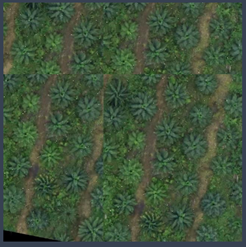
\includegraphics[width=0.4\columnwidth]{bab4/Gambar/tbl-5-pic7.png}\\ \hline
			
		\end{tabular}
	\end{table}
\end{singlespace}
%%%%%%%%%%%%%%%%%%%%%%%TABEL SEDERHANA%%%%%%%%%%%%%%%%%%%%%%%%%

Proses augmentasi dengan menambahkan 3987 citra tersimpan pada layanan roboflow yang digunakan citra untuk komputasi, yang terbagi untuk data pelatihan, validasi, dan pengujian dengan model CNN. Selanjutnya, untuk pembentukan dataset otomatis dengan memberikan anotasi atau pemberian label kelas secara otomatis pada objek di dalam citra dataset primer. Hal ini merupakan salah satu kebaruan pada penelitian ini dan proses tersebut dijelaskan pada sub bab \ref{sec:membangun-data}.

\subsection{Membersihkan Data}
\hspace{1,2cm}
Proses pada tahap membersihkan data dilakukan dengan memvalidasi data citra yang ditangkap pada dataset primer yang tidak dapat digunakan sebagai dataset. Proses ini dilakukan dengan validasi satu persatu dataset citra yang ditangkap oleh drone. Citra yang tidak digunakan merupakan citra yang ditangkap oleh drone tidak berada posisi yang tegak dari atas, tidak diambil dari sisi samping dari kamera drone dan tangkapan citra yang tidak terdapat pohon kelapa sawit. Terdapat 26 citra yang tidak dapat digunakan pada dataset primer sebagai citra untuk proses membangun data atau melakukan proses anotasi otomatis, seperti pada Gambar \ref{img:Data-Citra-Primer-Yang-Tidak-Digunakan}.

%%%%%%%%%%%%%%%%%%%%%%%%%% GAMBAR %%%%%%%%%%%%%%%%%%%%%%%%%%%%%%
\begin{figure}[H]
	\vspace{-0.1cm}
	%\rule{\columnwidth}{0.1pt}
	%\begin{center}
	%	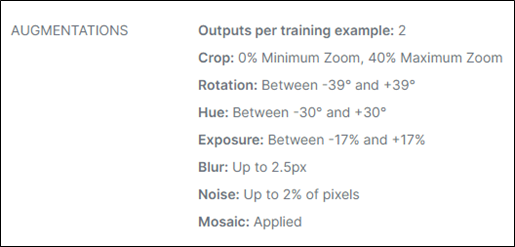
\includegraphics[width=1\columnwidth]{bab4/Gambar/Picture7.png}
	%\end{center}
	\centering
	\subfloat{{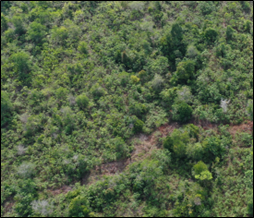
\includegraphics[width=6cm]{bab4/Gambar/Picture9.1.png} }}%
	\qquad
	\subfloat{{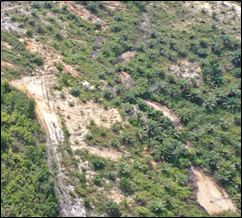
\includegraphics[width=6cm]{bab4/Gambar/Picture9.2.png} }}%
	\vspace{-0.2cm}
	%\rule{\columnwidth}{0.1pt}
	\captionsetup{justification=centering}
	\caption{Data Citra Primer yang tidak Digunakan (kiri: tidak terdapat pohon kelapa sawit; kanan: tampak area yang tidak tangkapan dari atas) }\label{img:Data-Citra-Primer-Yang-Tidak-Digunakan}
\end{figure}
%%%%%%%%%%%%%%%%%%%%%%%%%% GAMBAR %%%%%%%%%%%%%%%%%%%%%%%%%%%%%%

\subsection{Membangun Data}
\label{sec:membangun-data}
\hspace{1,2cm}
Proses anotasi otomatis merupakan pembentukan dataset berbasis OBIA. Proses anotasi ini digunakan dari data citra primer area studi Universitas Gunadarma di PPU, Kalimantan yaitu sebanyak 205 citra. Hasil dari 205 citra yang telah berhasil dideteksi sebagai objek pohon kelapa sawit ditampilkan dengan adanya \textit{bounding box} yang digunakan sebagai dataset untuk pelatihan dan pengujian model. Keluaran atau \textit{output} dari proses pembentukan dataset ini adalah citra yang dapat dideteksi objek di dalamnya sebagai pohon kelapa sawit yang dinyatakan dengan adanya \textit{bounding box} pada setiap objek yang terdeteksi yang memiliki data kelas, koordinat citra (x, y), dan \textit{width}, \textit{height} yang tersimpan dalam file dengan ekstensi *.txt.

Berdasarkan metode yang digunakan pada pembahasan bab 3 subbab \ref{sec:Deskripsi-Dataset-dan-Pemilihan-Data}, hal yang dilakukan pertama adalah menyiapkan pengumpulan data dalam satu folder yang sama. Data citra yang digunakan berupa 205 citra yang diambil oleh drone dari ketinggian 100 m dari permukaan tanah. Dalam penelitian ini, digunakan \textit{tools} atau peralatan berupa aplikasi \textit{jupyter notebook} untuk menuliskan kode program dan berbagi file dan berjalan di local komputer yang dijalankan pada web browser. Perintah yang digunakan dengan menggunakan \textit{command prompt} untuk mengaktifkan \textit{jupyter notebook}. Setelah berhasil aktif, maka diarahkan ke halaman homepage browser, dan dapat digunakan sebagai \textit{tools} untuk proses anotasi otomatis, seperti pada Gambar \ref{img:Home-Page-Jupyteer-Notebook}.

%%%%%%%%%%%%%%%%%%%%%%%%%% GAMBAR %%%%%%%%%%%%%%%%%%%%%%%%%%%%%%
\begin{figure}[H]
	\vspace{-0.1cm}
	\rule{\columnwidth}{0.1pt}
	\begin{center}
		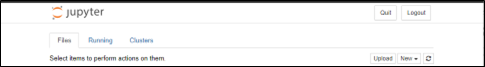
\includegraphics[width=1\columnwidth]{bab4/Gambar/Picture10.png}
	\end{center}
	\vspace{-0.2cm}
	%\rule{\columnwidth}{0.1pt}
	\captionsetup{justification=centering}
	\caption{\textit{Home Page} Jupyter Notebook}\label{img:Home-Page-Jupyteer-Notebook}
\end{figure}
%%%%%%%%%%%%%%%%%%%%%%%%%% GAMBAR %%%%%%%%%%%%%%%%%%%%%%%%%%%%%%

\subsection{Membuat Template}
\label{sec:Membuat-Template}
\hspace{1,2cm}
Tahap berikutnya dalam penelitian ini adalah membuat beberapa contoh gambar atau citra yang dijadikan sebagai template. Data citra yang digunakan berdimensi 5472 x 3078, maka pada jupyter notebook ditampilkan terlebih dahulu data citra untuk dapat ditampilkan citra yang digunakan untuk membuat template awal dengan sebuah fungsi. Data citra yang digunakan sebagai template seperti pada Gambar \ref{img:Data-Citra-Untuk-Membuat-Template}. 

%%%%%%%%%%%%%%%%%%%%%%%%%% GAMBAR %%%%%%%%%%%%%%%%%%%%%%%%%%%%%%
\begin{figure}[H]
	\vspace{-0.1cm}
	\rule{\columnwidth}{0.1pt}
	\begin{center}
		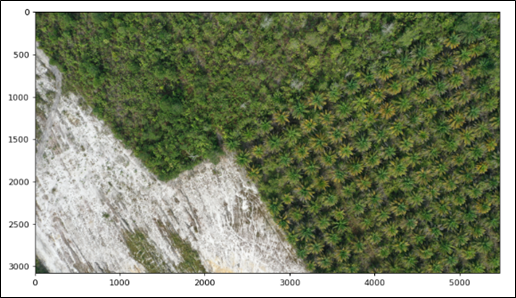
\includegraphics[width=1\columnwidth]{bab4/Gambar/Picture11.png}
	\end{center}
	\vspace{-0.2cm}
	%\rule{\columnwidth}{0.1pt}
	\captionsetup{justification=centering}
	\caption{Data citra untuk membuat template (5472 x 3078)}\label{img:Data-Citra-Untuk-Membuat-Template}
\end{figure}
%%%%%%%%%%%%%%%%%%%%%%%%%% GAMBAR %%%%%%%%%%%%%%%%%%%%%%%%%%%%%%

Dalam memudahkan pembuatan template gambar (objek kelapa sawit) digunakan fungsi \textit{onClick} untuk dapat menentukan beberapa titik tengah dari lokasi objek pohon kelapa sawit pada data citra. Dalam penelitian ini, digunakan 10 titik sebagai template objek. Titik yang dipilih merupakan objek citra pohon kelapa sawit yang ditandai dengan titik tengah merah yang berukuran 12 x 12 berdasarkan radius dari titik tengah yang telah ditentukan, seperti pada Gambar \ref{img:Membuat-Template-Yang-Ditandai}.

%%%%%%%%%%%%%%%%%%%%%%%%%% GAMBAR %%%%%%%%%%%%%%%%%%%%%%%%%%%%%%
\begin{figure}[H]
	\vspace{-0.1cm}
	\rule{\columnwidth}{0.1pt}
	\begin{center}
		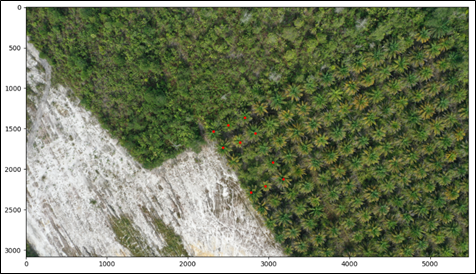
\includegraphics[width=1\columnwidth]{bab4/Gambar/Picture12.png}
	\end{center}
	\vspace{-0.2cm}
	%\rule{\columnwidth}{0.1pt}
	\captionsetup{justification=centering}
	\caption{Membuat Template yang Ditandai dengan Titik Objek Pohon Kelapa Sawit}\label{img:Membuat-Template-Yang-Ditandai}
\end{figure}
%%%%%%%%%%%%%%%%%%%%%%%%%% GAMBAR %%%%%%%%%%%%%%%%%%%%%%%%%%%%%%

Data citra berhasil ditampilkan dan ditandai dengan titik tengah merah untuk dijadikan sebagai template. Dalam pembuatan template ini, objek pohon kelapa sawit yang telah diberi titik dengan berwarna merah menjadi citra yang berukuran atau berdimensi 12 x 12 dari gambar asli. Citra tersebut ditampilkan dengan memiliki id dari 0 hingga 9 karena menggunakan array yang dimulai dari 0. Hal ini digunakan untuk dapat memudahkan penyesuaian titik tengah, jika terdapat titik yang tidak berada ditengah template yang diproses pada subbab 4.2.3.2. Gambar \ref{img:Citra-Template-Dari-Objek-Dari-Pohon-Kelapa-Sawit} hasil citra yang dijadikan sebagai template. 

%%%%%%%%%%%%%%%%%%%%%%%%%% GAMBAR %%%%%%%%%%%%%%%%%%%%%%%%%%%%%%
\begin{figure}[H]
	\vspace{-0.1cm}
	\rule{\columnwidth}{0.1pt}
	\begin{center}
		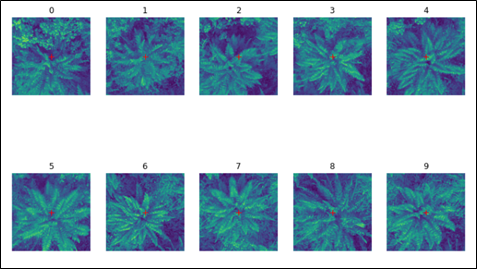
\includegraphics[width=1\columnwidth]{bab4/Gambar/Picture13.png}
	\end{center}
	\vspace{-0.2cm}
	%\rule{\columnwidth}{0.1pt}
	\captionsetup{justification=centering}
	\caption{Citra Template dari Objek Pohon Kelapa Sawit}\label{img:Citra-Template-Dari-Objek-Dari-Pohon-Kelapa-Sawit}
\end{figure}
%%%%%%%%%%%%%%%%%%%%%%%%%% GAMBAR %%%%%%%%%%%%%%%%%%%%%%%%%%%%%%

\subsubsection{Menyesuaikan Template}
\hspace{1,2cm}
Pada tahap ini, menyesuaikan template yang sudah tampak seperti pada gambar 4.10. Penyesuaian template adalah menyesuaikan titik tengah pada citra objek pohon kelapa sawit, jika titik tengah tidak berada pada tengah objek di citra tersebut. Penyesuaian ini dapat dilakukan dengan fungsi yang diterapkan, dan titik dapat dikoreksi dengan bergeser ke atas, bawah, kiri atau kanan dengan sebuah fungsi. Misalnya, pada id 2, titik tengah dari citra template tersebut yang ditandai dengan titik merah tidak berada di tengah, maka dapat digunakan fungsi turun (ke bawa) agar titik tersebut berada di tengah pohon kelapa sawit. Dalam penelitian ini dilakukan dengan 2 piksel setiap satu fungsi yang dijalankan untuk menggeser titik ke atas, bawah, kiri, atau kanan. Hasil koreksi dari menyesuaikan template untuk ID 2 ditampilkan pada Gambar \ref{img:Menyesuaikan-Template-Pada-ID-2}.

%%%%%%%%%%%%%%%%%%%%%%%%%% GAMBAR %%%%%%%%%%%%%%%%%%%%%%%%%%%%%%
\begin{figure}[H]
	\vspace{-0.1cm}
	\rule{\columnwidth}{0.1pt}
	\begin{center}
		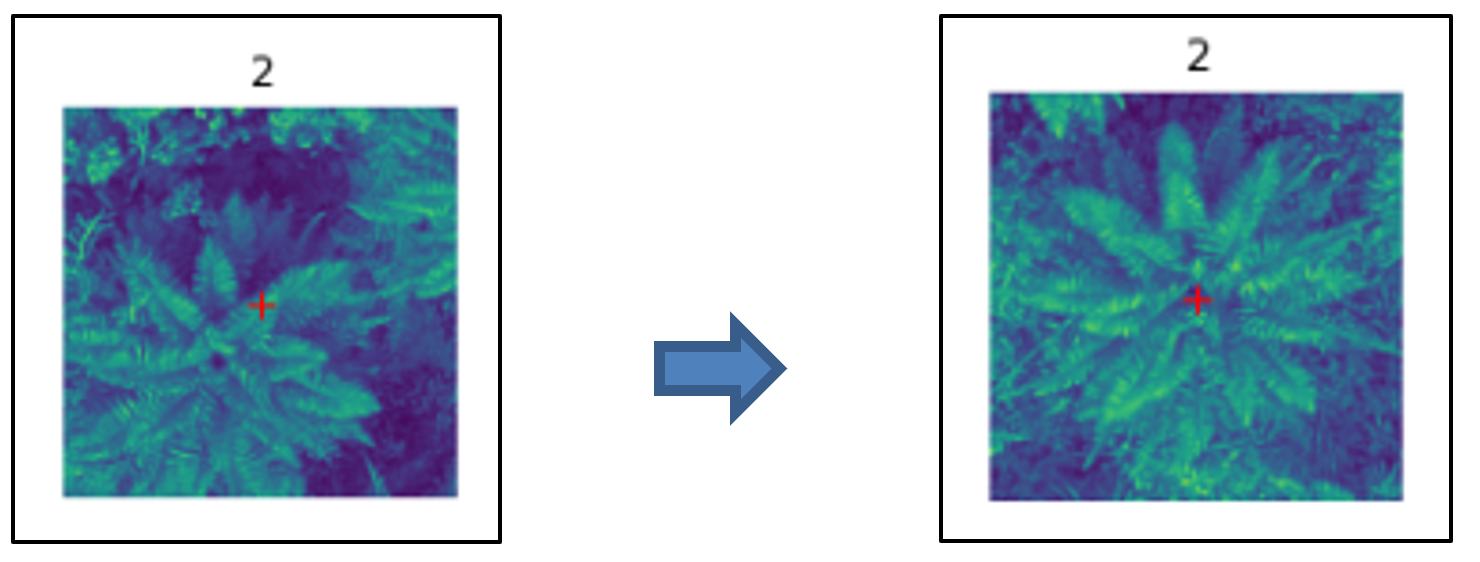
\includegraphics[width=1\columnwidth]{bab4/Gambar/Picture14.png}
	\end{center}
	\vspace{-0.2cm}
	%\rule{\columnwidth}{0.1pt}
	\captionsetup{justification=centering}
	\caption{Menyesuaikan Template pada ID 2}\label{img:Menyesuaikan-Template-Pada-ID-2}
\end{figure}
%%%%%%%%%%%%%%%%%%%%%%%%%% GAMBAR %%%%%%%%%%%%%%%%%%%%%%%%%%%%%%

\subsubsection{Evaluasi Korelasi diantara Template}
\hspace{1,2cm}
Ketika proses penyesuaian template selesai, maka pada tahap berikutnya adalah mengevaluasi korelasi antar template yang telah dibuat. Masing-masing template awal dibuat sebanyak 10 citra yang menunjukkan objek pohon kelapa sawit dengan dimensi 12 x 12. Dimensi 12 x 12 digunakan agar citra objek pohon kelapa sawit dapat terlihat lebih jelas yang menadakan 1 (satu) objek pohon kelapa sawit yang dipilih sebagai template. Berdasarkan perhitungan yang dilakukan pada persamaan 6 - 9 pada sub bab 3.3.3.3 didapatkan hasil korelasi diantara template dan waktu yang dibutuhkan untuk mengkalkulasi korelasi template tersebut pada Tabel \ref{tbl:Hasil-Rerata-Korelasi-dan-Waktu-Yang-Dibutuhkan}.

%%%%%%%%%%%%%%%%%%%%%%%TABEL SEDERHANA%%%%%%%%%%%%%%%%%%%%%%%%%
\begin{singlespace}
	\begin{table}[H]
		\centering
		\caption{Hasil Rerata Korelasi dan Waktu yang Dibutuhkan}
		\label{tbl:Hasil-Rerata-Korelasi-dan-Waktu-Yang-Dibutuhkan}
		\begin{tabular}{|p{8cm}|p{4cm}|}
			\hline
			\rowcolor[HTML]{D9D9D9} 
			Deskripsi                                 & Nilai \\ \hline
			Evaluasi korlasi diantara template        & 0.16  \\ \hline
			Waktu yang dibuthkan untuk menghitung (d) & 57    \\ \hline
		\end{tabular}
	\end{table}
\end{singlespace}
%%%%%%%%%%%%%%%%%%%%%%%TABEL SEDERHANA%%%%%%%%%%%%%%%%%%%%%%%%%

Berdasarkan Tabel \ref{tbl:Hasil-Rerata-Korelasi-dan-Waktu-Yang-Dibutuhkan}. terlihat bahwa waktu yang dibutuhkan untuk menghitung nilai rata-rata korelasi antar template membutuhkan waktu sebanyak 57 detik, dan nilai korelasi citra dihasilkan sebesar 0.16. Hal ini menunjukkan nila ikorelasi citra baik, karena nilai korelasi berada di rentang -1 sampai + 1. Jika nilai mendekati 1, maka nilai ini sebagai ambang batas untuk digunakan dalam metode atau algoritma \textit{template matching} untuk mendeteksi keberadaan objek kelapa sawit pada citra yang dapat diberikan anotasi atau label pohon kelapa sawit untuk dijadikan dataset.

\subsubsection{Penambahan Template}
\hspace{1,2cm}
Nilai korelasi antar template sudah diketahui, Langkah selanjutnya dilakukan menambahkan template dari 10 citra yang sudah dimiliki sebagai template. Hal ini digunakan untuk menambahkan data citra yang diproses pada \textit{template matching}, sehingga metode dapat digunakan dengan mengenali berbagai data citra sebagai template bahwa citra tersebut adalah objek pohon kelapa sawit. 

Pada penambahan template ini digunakan rotasi sebesar 30$^{\circ}$ (tiga puluh derajat), yang dimana setiap 1 gambar sebanyak 4 (empat kali) dirotasi sebesar 30$^{\circ}$. Hasil citra template yang sudah di rotasi seperti pada Gambar \ref{img:Hasil-Rotasi-30}. 

%%%%%%%%%%%%%%%%%%%%%%%%%% GAMBAR %%%%%%%%%%%%%%%%%%%%%%%%%%%%%%
\begin{figure}[H]
	\vspace{-0.1cm}
	\rule{\columnwidth}{0.1pt}
	\begin{center}
		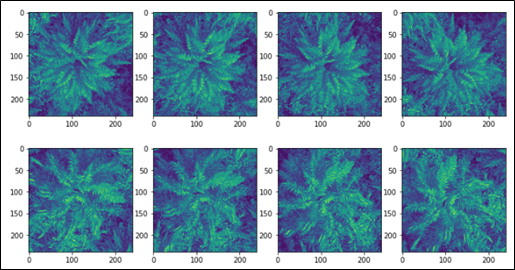
\includegraphics[width=1\columnwidth]{bab4/Gambar/Picture15.png}
	\end{center}
	\vspace{-0.2cm}
	%\rule{\columnwidth}{0.1pt}
	\captionsetup{justification=centering}
	\caption{Hasil Rotasi 30$^{\circ}$ pada Citra template}\label{img:Hasil-Rotasi-30}
\end{figure}
%%%%%%%%%%%%%%%%%%%%%%%%%% GAMBAR %%%%%%%%%%%%%%%%%%%%%%%%%%%%%%

Proses untuk mendapatkan citra yang di rotasi untuk 10 (sepuluh) citra template tampak seperti pada Tabel \ref{tbl:Waktu-Yang-Dibutuhkan-Untuk-Rotasi}. 

%%%%%%%%%%%%%%%%%%%%%%%TABEL SEDERHANA%%%%%%%%%%%%%%%%%%%%%%%%%
\begin{singlespace}
	\begin{table}[H]
		\centering
		\caption{Waktu yang Dibutuhkan untuk Rotasi}
		\label{tbl:Waktu-Yang-Dibutuhkan-Untuk-Rotasi}
		\begin{tabular}{|p{8cm}|p{4cm}|}
			\hline
			\rowcolor[HTML]{D9D9D9} 
			Deskripsi                                  & Nilai \\ \hline
			Waktu yang dibutuhkan untuk rotasi (detik) & 8 \\ \hline
		\end{tabular}
	\end{table}
\end{singlespace}
%%%%%%%%%%%%%%%%%%%%%%%TABEL SEDERHANA%%%%%%%%%%%%%%%%%%%%%%%%%

\subsubsection{Menjalankan Template Matching}
\hspace{1,2cm}
Pada tahap ini dilakukan match template yaitu anotasi secara otomatis dengan mendeteksi (klasifikasi) mengenali adanya objek pohon kelapa sawit pada citra. Citra utuh yang besar (gambar asli) dideteksi menjadi bagian-bagian yang terdeteksi menjadi citra yang dikenali sebagai objek yang menjadi dataset. Gambar yang terdeteksi dengan \textit{template matching} ini dideteksi dengan lingkarran merah pada Gambar \ref{img:Objek-Yang-Terdeteksi-Untuk-Dataset}.

%%%%%%%%%%%%%%%%%%%%%%%%%% GAMBAR %%%%%%%%%%%%%%%%%%%%%%%%%%%%%%
\begin{figure}[H]
	\vspace{-0.1cm}
	\rule{\columnwidth}{0.1pt}
	\begin{center}
		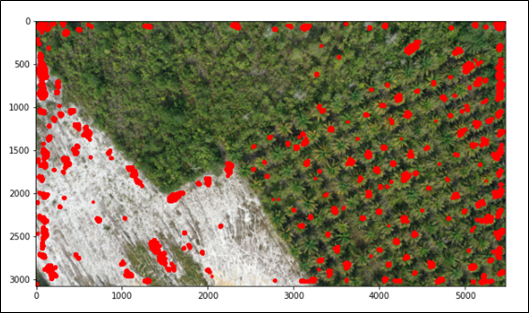
\includegraphics[width=1\columnwidth]{bab4/Gambar/Picture16.png}
	\end{center}
	\vspace{-0.2cm}
	%\rule{\columnwidth}{0.1pt}
	\captionsetup{justification=centering}
	\caption{Objek yang terdeteksi untuk Dataset dengan \textit{Template Matching}}\label{img:Objek-Yang-Terdeteksi-Untuk-Dataset}
\end{figure}
%%%%%%%%%%%%%%%%%%%%%%%%%% GAMBAR %%%%%%%%%%%%%%%%%%%%%%%%%%%%%%

Gambar \ref{img:Objek-Yang-Terdeteksi-Untuk-Dataset}. yang terdeteksi terlihat seperti adanya tumpang tindih atau mungkin tidak seperti pohon kelapa sawit yang merupakan dataset yang diharapkan, karena nilai ambang batas (\textit{threshold}) dibatasi pada nilai rata-rata nilai korelasi diantara template yang lebih rendah, sehingga ketika berada di atas nilai korelasi, maka terdeteksi sebagai citra yang cocok dengan template.

\subsubsection{Analisis Cluster dengan BIRCH}
\hspace{1,2cm}
Tahap ini dilakukan setelah berhasil dideteksi dengan menggunakan \textit{template matching}, selanjutnya dilakukan analisis cluster dengan algoritma BIRCH untuk mereduksi atau mencari nilai ambang batas dari citra yang tidak sesuai berdasarkan nilai mean r (korelasi). Pada BIRCH ini digunakan nilai ambang batas (\textit{threshold}) secara acak yang digunakan sebagai nilai ambang batas minimum yang dimasukkan ke dalam citra untuk dapat mendeteksi objek yang terdeteksi pohon kelapa sawit pada citra yang sudah dideteksi dengan \textit{template matching}. Nilai ambang batas (threshold) yang digunakan dalam penelitian ini adalah 0.5. Hasil objek yang terdeteksi sebagai pohon kelapa sawit pada citra untuk menjadi dataset ditampilkan dengan kotak batas (\textit{bounding box}) dengan kotak berwarna merah. Hal ini menujukkan bahwa kotak tersebut mendeteksi objek pohon kelapa sawit yang tampak seperti pada Gambar \ref{img:Hasil-Objek-Yang-Terdeteksi}.

%%%%%%%%%%%%%%%%%%%%%%%%%% GAMBAR %%%%%%%%%%%%%%%%%%%%%%%%%%%%%%
\begin{figure}[H]
	\vspace{-0.1cm}
	\rule{\columnwidth}{0.1pt}
	\begin{center}
		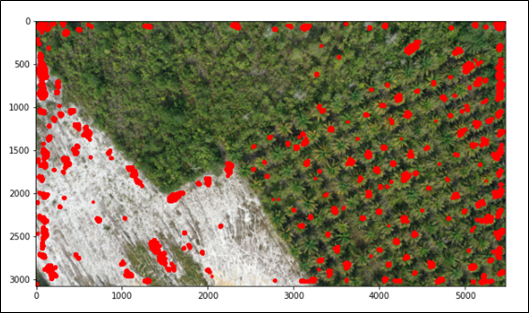
\includegraphics[width=1\columnwidth]{bab4/Gambar/Picture16.png}
	\end{center}
	\vspace{-0.2cm}
	%\rule{\columnwidth}{0.1pt}
	\captionsetup{justification=centering}
	\caption{Hasil objek yang terdeteksi untuk Dataset dengan algoritma BIRCH}\label{img:Hasil-Objek-Yang-Terdeteksi}
\end{figure}
%%%%%%%%%%%%%%%%%%%%%%%%%% GAMBAR %%%%%%%%%%%%%%%%%%%%%%%%%%%%%%

Berdasarkan Gambar \ref{img:Objek-Yang-Terdeteksi-Untuk-Dataset} diketahui template matching dari citra berhasil mendeteksi objek untuk dataset, namun masih terjadi tumpang tindih atau overlapping dan berdasarkan hasil dari algoritma BIRCH pada Gambar \ref{img:Hasil-Objek-Yang-Terdeteksi}., dihasilkan pengurangan nilai dan terdeteksi objek pohon kelapa sawit pada citra. Hasil waktu yang digunakan untuk mendeteksi objek sebagai dataset ditunjukkan pada Tabel \ref{tbl:Hasil-Waktu-Yang-Dibutuhkan-Untuk-Deteksi-Objek-Sebagai-Dataset}.

%%%%%%%%%%%%%%%%%%%%%%%TABEL SEDERHANA%%%%%%%%%%%%%%%%%%%%%%%%%
\begin{singlespace}
	\begin{table}[H]
		\centering
		\caption{Hasil Waktu yang Dibutuhkan untuk Deteksi Objek sebagai Dataset}
		\label{tbl:Hasil-Waktu-Yang-Dibutuhkan-Untuk-Deteksi-Objek-Sebagai-Dataset}
		\begin{tabular}{|m{5cm}|m{3cm}|m{4cm}|}
			\hline
			\rowcolor[HTML]{D9D9D9} 
			Deskripsi                                    & Waktu (detik) & Jumlah yang Terdeteksi \\ \hline
			Waktu yang dibutuhkan pada Template Matching & 334              & 463                    \\ \hline
			Waktu yang dibutuhkan pada BIRCH             & 24               & 148                    \\ \hline
		\end{tabular}
	\end{table}
\end{singlespace}
%%%%%%%%%%%%%%%%%%%%%%%TABEL SEDERHANA%%%%%%%%%%%%%%%%%%%%%%%%%

Berdasarkan hasil Tabel \ref{tbl:Hasil-Waktu-Yang-Dibutuhkan-Untuk-Deteksi-Objek-Sebagai-Dataset}. diketahui bahwa \textit{template matching} membutuhkan waktu 334 detik untuk berhasil mendeteksi 463 objek, sedangkan dengan BIRCH membutuhkan waktu 24 detik dan berhasil direduksi untuk menemukan nilai ambang batas yang baik menjadi 148 yang terdeteksi sesuai dengan nilai yang telah ditentukan. 

\subsubsection{Menjalankan Auto-Annotate Datasets}
\hspace{1,2cm}
Proses dengan \textit{template matching} dan BIRCH berhasil dideteksi objek pada citra yang ditampilkan dengan \textit{bounding box}. Tahap selanjutnya menjalankan anotasi otomatis. Proses ini mengambil data citra sebanyak 205 citra dari data primer yang berada dalam 1 folder, kemudian dijalankan proses tersebut. Proses ini mendeteksi objek yang sesuai sebagai pohon kelapa sawit pada citra, sehingga dapat dikenali dan diperoleh kelas, koordinat x, koordinat y, \textit{width}, \textit{height} disimpan dalam file berekstensi *.txt (sesuai nama file citra). File merupakan hasil dari proses anotasi dataset yang berisi kelas, koordinat x, koordinat y, \textit{width}, \textit{height}.

Berdasarkan hasil anotasi otomatis membutuhkan waktu yang signifikan untuk membuat dataset dengan anotasi otomatis dari citra yang berjumlah 205. Waktu yang dibutuhkan proses ini seperti terlihat pada Tabel 4.9.

%%%%%%%%%%%%%%%%%%%%%%%TABEL SEDERHANA%%%%%%%%%%%%%%%%%%%%%%%%%
\begin{singlespace}
	\begin{table}[H]
		\centering
		\caption{Hasil Waktu Yang Dibutuhkan untuk Anotasi Otomatis}
		\label{tbl:Hasil-Waktu-Yang-Dibutuhkan-Untuk-Anotasi-Otomatis}
		\begin{tabular}{|m{10cm}|m{2cm}}
			\hline
			\rowcolor[HTML]{D9D9D9} 
			Deskripsi                                            & Waktu (mm:dd) \\ \hline
			Waktu yang dibutuhkan untuk Anotasi Otomatis Dataset & 30:24         \\ \hline
		\end{tabular}
	\end{table}
\end{singlespace}
%%%%%%%%%%%%%%%%%%%%%%%TABEL SEDERHANA%%%%%%%%%%%%%%%%%%%%%%%%%

Berikut ini adalah contoh hasil anotasi otomatis pada file berekstensi *.txt yang berisi kelas, koordinat x, koordinat y, width, dan height terlihat pada Gambar 4.18.

%%%%%%%%%%%%%%%%%%%%%%%%%% GAMBAR %%%%%%%%%%%%%%%%%%%%%%%%%%%%%%
\begin{figure}[H]
	\vspace{-0.1cm}
	%\rule{\columnwidth}{0.1pt}
	\begin{center}
		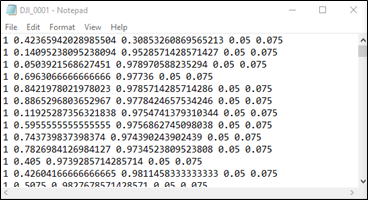
\includegraphics[width=0.6\columnwidth]{bab4/Gambar/Picture18.1.png}
		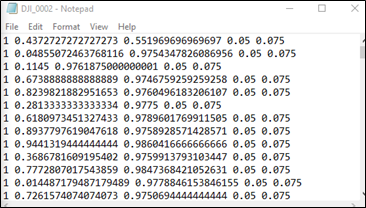
\includegraphics[width=0.6\columnwidth]{bab4/Gambar/Picture18.2.png}
	\end{center}
	\vspace{-0.2cm}
	%\rule{\columnwidth}{0.1pt}
	\captionsetup{justification=centering}
	\caption{Hasil Anotasi Otomatis dalam format file *.txt}\label{img:Hasil-Anotasi-Otomatis}
\end{figure}
%%%%%%%%%%%%%%%%%%%%%%%%%% GAMBAR %%%%%%%%%%%%%%%%%%%%%%%%%%%%%%

Pada Gambar \ref{img:Hasil-Anotasi-Otomatis}. terdapat 5 bilangan berurutan, nilai ke-1 menunjukkan bilangan yang sama, untuk digunakan sebagai kelas yang terdeteksi yaitu kelas 'oil palm', untuk barisan ke-2, ke-3, ke-4, dan ke-5 masing-masing menunjukkan koordinat x, koordinat y, lebar dan tinggi. Lebar dan tinggi dapat terlihat sama, karena dataset memiliki karakteristik dimensi ukuran citra yang sama.

Setelah itu, pada penelitian ini dilakukan pengujian dengan 10 citra yang dapat dilihat pada Tabel 4.10.

TABEL TABEL

Berdasarkan hasil pengujian terhadap 10 citra dari hasil pada Tabel 4.10 didapatkan rata-rata akurasi yang terdeteksi pada penelitian ini sebesar 89.90\% dengan menggunakan metode \textit{template matching} dan algoritma BIRCH. Hal ini menunjukkan hal penting yang signifikan yang harus dilakukan dalam proses anotasi otomatis yang dapat digunakan untuk memberikan deteksi gambar yang lebih akurat dan lebih cepat.

Setelah dilakukan pengujian dan juga dilakukan anotasi otomatis dari citra dan deteksi objek pohon kelapa sawit, maka citra yang tersimpan pada folder di local komputer beserta format file *.txt yang merupakan dataset. Hasil tersebut seperti pada Gambar 4.19.

GAMBAR GAMBAR

\subsubsection{Integrasi Data}
\hspace{1,2cm}
Proses integrasi data dilakukan untuk menggabungkan atau menyatukan dua dataset, yaitu dataset primer dan sekunder ke dalam satu sumber. Dataset sekunder digunakan layanan roboflow untuk menampung data yang sudah tersimpan pada layanan tersebut. Selanjutnya, hasil dari pembangunan dataset dengan anotasi atau pelabelan otomatis yang telah dilakukan, maka diunggah data citra dan file *.txt. 


GAMBAR 20


Pada Gambar 4.20. terlihat kumpulan gambar sebanyak 205 gambar yang menandakan bahwa dataset dari citra asli sebanyak 205 berhasil terunggah, dan satu citra dapat memiliki lebih dari objek pohon kelapa sawit dengen kelas 'oil palm' pada satu citra. 

Pada Gambar 4.20 dan 4.21 terlihat kotak pembatas atau yang dikenal dengan nama \textit{bounding box} yang berwarna hijau, hal ini menandakan objek yang terdeteksi sebagai dataset. Setiap 1 citra dataset primer memiliki jumlah \textit{bounding box} yang berbeda-beda karena tergantung hasil yang dideteksi, seperti pada Gambar 4.21 terdapat 414 objek pohon kelapa sawit yang terdeteksi dalam anotasi atau label dari 1 citra. 

GAMBAR 21

Berdasarkan hasil yang telah dilakukan pada pembentukan dataset secara otomatis dengan pendekatan OBIA berhasil dilakukan, dan citra yang menjadi dataset primer dapat digunakan dan di integrasikan (digabungkan) dengan dataset sekunder untuk komputasi. 

\subsubsection{Format Data}
\hspace{1,2cm}
Pada proses ini dilakukan format data primer dan sekunder dengan menggunakan bantuan layanan roboflow sebelum dapat digunakan untuk citra komputasi yang dibagi menjadi dataset pelatihan, validasi, dan test.  Pada tahap ini menyesuaikan tipe data pada citra yaitu pada dataset primer dan sekunder sama-sama *.jpg, dan mengurangi dimensi dataset citra dengan melakukan resize citra menjadi 640 x 640, seperti pada Gambar 4.22. 

GAMBAR 22

Ketika proses pada Gambar 4.22 sudah dilakukan, maka selanjutnya dataset yang telah sesuai dengan format data yang ditentukan dapat digunakan untuk citra komputasi. Dataset dipindahkan ke layanan Google Drive untuk kemudian dilakukan citra komputasi yang membagi data untuk data pelatihan, validasi dan pengujian sesuai dengan fold yang digunakan, yaitu sebanyak 5 fold (dengan nama dataset folds 0 sampai 4) seperti Gambar 4.23.

\section{Citra untuk Komputasi}
\hspace{1,2cm}
Pada tahap ini citra gambar untuk komputasi merupakan kumpulan dari citra dataset primer dan sekunder. Jumlah dataset sebanyak 6056 data, yang terbagi ke dalam 78\% data pelatihan, 20\% data validasi dan 2\% data pengujian, seperti pada Tabel 4.11.

TABEL 11

Dataset tersebut dikumpulkan atau digabungkan, serta dibagi menjadi 5 bagian. Karena pada proses pelatihan dan pengujian mengunakan teknik evaluasi K-Fold Cross-Validation. Berikut ini contoh citra yang digunakan dengan file *.txt yang berisi anotasi objek yang digunakan untuk dataset pelatihan, dataset validasi, dan dataset pengujian seperti tampak pada Gambar 4.24.

GAMBAR 24 ADA 6

\section{Pelatihan Model CNN}
\hspace{1,2cm}
Pada proses pelatihan ini dengan menggunakan model CNN pada YOLOv5, YOLOv6, dan YOLOv7 yang divalidasi dengan menggunakan K-Fold Cross-Validation, dimana semua bagian dataset dapat digunakan untuk pelatihan dan pengujian. Teknik ini digunakan untuk evaluasi performance dari model untuk mengurangi overfitting.  Pada penelitian ini menggunakan k = 5, dimana proses ini diulang sebanyak k = 5 kali. Setiap fold masing-masing terdiri dari data pelatihan yang merupakan gabungan dari data pelatihan sebanyak 4744 data dan 1187 validasi, untuk data test sebanyak 125 data citra. Setiap fold berisi data ini untuk dapat diketahui pada fold mana hasil model yang dilatih hasilnya lebih baik. Pada proses pelatihan ini data citr auntuk dataset dikonversi untuk data masukkan gambar pada proses pelatihan dengan menggunakan ukuran gambar yang diatur oleh YOLO, yaitu secara default 640 x 640. Pada pelatihan model dan pengujian menggunakan parameter optimasi seperti pada Tabel 4.12.

TABEL 4.12

Pada pelatihan menggunakan mesin pada Google Colab Pro dan DGX-A-100 yang dimiliki oleh Universitas Gunadarma. Mesin NVIDIA yang digunakan, seperti pada Tabel 4.13. 


TABEL 4.13

Pelatihan model CNN pada penelitian ini menggunakan validasi performance yang menghasilkan 4 hasil yang berbeda dengan menggunakan \textit{Precision}, \textit{Recall}, \textit{F1-Score}, dan \textit{best mean Average Precision} atau best mAP@0.5.

\subsection{Pelatihan Model CNN YOLOv5}
\hspace{1,2cm}
Pelatihan model pertama dilatih dengan menggunakan YOLOv5. Pada Tabel 4.13 hasil pelatihan model CNN dengan YOLOv5 dengan 30 epoch dan batch size 16 pada Google Colab Pro. Pada mesin DGX-A-100 milik Universitas Gunadarma dengan menggunakan batch size sebesar 16 tidak dapat dijalankan karena permasalahan \textit{suificient memory} (runs out memory) atau kehabisan shared virtual memori untuk dapat digunakan, sehingga menggunakan batch size dibawahnya dalam 1 iterasi, yaitu 10. Hasil evaluasi model menunjukkan hasil yang cukup signifikan bahwa rata-rata dengan hasil pelatihan dengan Google Colab Pro lebih baik dibandingkan dengan hasil DGX A 100, berturut turut \textit{Precision}, \textit{Recall}, \textit{F1-Score}, best mAP@0.5. Adalah 0,957, 0,955, 0,955 dan 0,974, sedangkan dengan menggunakan DGX-A100 sedikit menurun yaitu 0,949, 0,955, 0,955, dan 0,974, hal ini karena memory pemrosesan dan penggunaan GFlops pada saat pelatihan model. Hasil Fold evaluasi pelatihan model dengan YOLOv5 tampak pada Tabel 4.14.

Hasil pelatihan terbaik ditampilkan pada fold ke-4 dengan menggunakan mesin Goole Collab Pro. 